\chapter{Dataset analysis and preparation}\label{ch:data-ana}

As mentioned in \Cref{ch:intro}, the dataset used in this thesis is the Indoor Location \& Navigation from kaggle \cite{kaggle}, which was part of a competition of Microsoft Research in 2021 \cite{IndoorLocationNavigation}.
The company \(XYZ^{10}\) recorded the data in shopping malls and was provided by Microsoft Research for this competition.
The goal for the competition was to give a file with a path of a shopping mall and predict the floor and waypoint locations at a timestamp given in the submission files for that shopping mall.
The following will analyze and prepare the dataset and data for the \ac{ml} model.


\section{Components of the dataset}\label{sec:data}
As noted in the kaggle notebook ``Indoor Navigation: Complete Data Understanding'' \cite{IndoorNavigationUnderstanding} the data consists of 3 parts:

\begin{itemize}
    \item a train folder with train path files, organized by site and floor
    \item a test folder with test path files, organized by site and floor but without waypoint data
    \item a metadata folder with floor metadata, organized by site and floor, which includes floor images, further information, and a geojson map
\end{itemize}

The train folder contains 204 subfolders representing each site where the data was recorded.
In each site folder are a minimum of one and a maximum of twelve subfolders, which represent the floors of the site; the median is five floors.
Overall, there are 26,925 files, each containing the movement of one person for a specific site and floor.
Per floor, there are between one and 284 files with a median of 14.
The floor F1 of the site \begin{CJK*}{UTF8}{gbsn}银泰城(城西店)\end{CJK*} (Yintai City (Chengxi Branch)) which was hashed as ``5d27075f03f801723c2e360f'' in the train folder of the competition, has the most files.

The submission files and the test folder will not be used for this thesis.
Instead, we will generate our test set out of the train data because our goal is not to predict the floor and site name for a specific timestamp but to predict the \ac{bssid} to which a device may connect next, which is an entirely different task.
Therefore, we will not analyze the content of the test and metadata folders in detail.


\section{File structure}\label{sec:file-structure}

Each file in each floor folder is a \textbf{.txt} file. 
The first two lines and the last are denoted with ``\#''.
The first contains the start time of the recording, the second site information SiteID as hash, SiteName, FloorId as hash, and FloorName.
The last line contains the end time of the recording.
The central part of the data consists of the collected data. 
Each line contains a UNIX timestamp in milliseconds, followed by a data type and the data itself, all separated by a tabulator.
The GitHub repository of the competition \cite{GitHubComp} shows that the data type in the second column followed by its data can be one of the following:

\setlist[enumerate]{label=(\arabic*)}
\begin{enumerate}
    \item\label{type:acce} TYPE\_ACCELEROMETER with x, y and z acceleration and an accuracy value
    \item\label{type:mag} TYPE\_MAGNETIC\_FIELD with x, y and z magnetic field and an accuracy value
    \item\label{type:gyro} TYPE\_GYROSCOPE with x, y and z gyroscope and an accuracy value
    \item\label{type:rot} TYPE\_ROTATION\_VECTOR with x, y and z rotation vector and an accuracy value
    \item\label{type:mag_u} TYPE\_MAGNETIC\_FIELD\_UNCALIBRATED with x, y and z magnetic field and an accuracy value
    \item\label{type:gyro_u} TYPE\_GYROSCOPE\_UNCALIBRATED with x, y and z gyroscope and an accuracy value
    \item\label{type:acce_u} TYPE\_ACCELEROMETER\_UNCALIBRATED with x, y and z acceleration and an accuracy value
    \item\label{type:wifi} TYPE\_WIFI with \ac{ssid}, \ac{bssid}, \ac{rssi}, frequency, and last seen timestamp of the access point. The SSID and BSSID are hashed.
    \item\label{type:beacon} TYPE\_BEACON with \ac{uuid}, \ac{MajorID}, \ac{MinorID}, \ac{TxPower}, \ac{rssi}, distance to the device measured by the beacon, \ac{mac} address and a timestamp as padding data. The MajorID and MinorID are hashed.
    \item\label{type:way} TYPE\_WAYPOINT with x and y coordinates, which are the ground truth locations labeled by the surveyor
\end{enumerate}

\lstset{
    basicstyle=\scriptsize\ttfamily,
    breaklines=true,
    escapeinside={(*@}{@*)},
}

\begin{lstlisting}[caption={A snippet from the dataset of the file 5daa9e38df065a00069beb79.txt of the floor F4},label={lst:dataset}]
    #   startTime:1571462193934
    #   SiteID:5d27099303f801723c32364d SiteName:(*@\begin{CJK*}{UTF8}{gbsn}银泰百货(庆春店)\end{CJK*}@*) FloorId:5d27099303f801723c323650 FloorName:4F
    1571462193944   TYPE_WAYPOINT   57.885998   69.501526
    1571462194071   TYPE_ACCELEROMETER  -0.95254517 0.7944031   8.928757    2
    1571462194071   TYPE_MAGNETIC_FIELD -25.65918   -4.4784546  -28.201294  3
    1571462194071   TYPE_GYROSCOPE  -0.22373962 -0.07733154 -0.16847229 3
    1571462194071   TYPE_ROTATION_VECTOR    0.04186145  -0.02101801 -0.72491926 3
    1571462194071   TYPE_MAGNETIC_FIELD_UNCALIBRATED    -4.8568726  10.406494   -387.44965  20.802307   14.884949   -359.24835  3
    1571462194071   TYPE_GYROSCOPE_UNCALIBRATED -0.22218323 -0.068359375    -0.1628418  0.0026245117    9.765625E-4 -7.6293945E-4   3
    1571462194071   TYPE_ACCELEROMETER_UNCALIBRATED -0.95254517 0.7944031   8.928757    0.0 0.0 0.0 3
    ...
    1571462194883   TYPE_WIFI   b06c4e327882fab58dfa93ea85ca373a54e887b5    9f967858afcbb907af6e5adef766c7e7b936ef07    -63 2462    1571462190744
    1571462194883   TYPE_WIFI   8204870beb9d02995dab3f08aad97af5eab723cc    0413b35df78fc865af15b4721d5aeb33ff57da45    -64 2447    1571462188686
    ...
    1571462194020   TYPE_BEACON 07efd69e3167537492f0ead89fb2779633b04949    b6589fc6ab0dc82cf12099d1c2d40ab994e8410c    76e907e391ad1856762f70538b0fd13111ba68cd    -57 -71 5.002991815535578   1b7e1594febd760b00f1a7984e470867616cee4e    1571462194020
    ...
    1571462195943   TYPE_WAYPOINT   59.72475    69.02152
    #   endTime:1571462195976
\end{lstlisting}

Each file contains a different amount of waypoints and sensor data.
Each file's first and last data type is a \ref{type:way}.
Lines with types from \ref{type:acce} to \ref{type:acce_u} occur every 20 ms and are measured at the same time.
\ref{type:wifi} occurs about every 1800-2200 ms.
\ref{type:way} data is not evenly distributed.
An assumption for this is that the recording of the waypoint data is triggered by an exterior event, e.g., a button press.
As seen in \Cref{lst:dataset}, the data are measured separately from each other, so there are no combinations of the data types.

A prediction of the next \ac{bssid} will only work per site due to the different \acp{ap} and, therefore, \acp{bssid} per site.
Still, the prediction could be difficult for a whole site because the \acp{ap} are different on each floor, which may result in many \acp{ap} for the prediction.
To better predict, we will focus on a single floor of a site and use the data from the fourth floor of the shopping mall in Yintai City (Chengxi Branch).
To further know how much data we have for the model, \Cref{tab:data_summary} shows a more detailed analysis.
% \subsection{Analysis of floor with most files}
\begin{table}[h]
    \centering
    \caption{Summary of data for F1 of site Yintai City (Chengxi Branch)}
    \begin{tabular}{|l|l|}
    \hline
    \textbf{Information} & \textbf{Value} \\ \hline
    Total data points & 7,157,081 \\ \hline
    Average data points per file & 25,201 \\ \hline
    Number of waypoints & 2,027 \\ \hline
    Lines of each \ref{type:acce} to \ref{type:acce_u} data & 746,689 \\ \hline
    Lines of \ac{wifi} data & 1,862,044 \\ \hline
    Lines of beacon data & 66,187 \\ \hline
    Number of \acp{bssid} & 4,795 \\ \hline
    Number of \acp{ap} & 4,795 \\ \hline
    Number of \acp{ssid} & 1,421 \\ \hline
    \ac{rssi} range & -93 to -13 dBm \\ \hline
    \end{tabular}
\label{tab:data_summary}
\end{table}


\section{Preprocessing data for an ML model}\label{sec:prep-on-data-for-an-ml-model}

As seen in previous sections, a location for the time of \texttt{TYPE\_WIFI} data points is not provided.
Also, we have 2,027 waypoints for this floor but 1,862,044 lines of \ac{wifi} data, as seen in \Cref{tab:data_summary}.
The visualization of the waypoints can be seen in \Cref{fig:vis-wo-interpolated}.

\begin{figure}[h!]
    \centering
    \includegraphics[scale=0.375]{images/whole_floor_visualization_wo_interpolated.pdf}
    \caption{Visualization of the 2,027 waypoints of the site Yintai City (Chengxi Branch) on floor F1}
    \label{fig:vis-wo-interpolated}
\end{figure}

Further human movement between \texttt{TYPE\_WAYPOINT} and \texttt{TYPE\_WIFI} data points may have occurred.
Therefore, we cannot combine the data points directly to get a location for the \ac{wifi} data points.
Nevertheless, they can be combined using linear interpolation.%, as seen in \Cref{fig:interpolation}.

% \begin{figure}[h!]
%     \centering
%     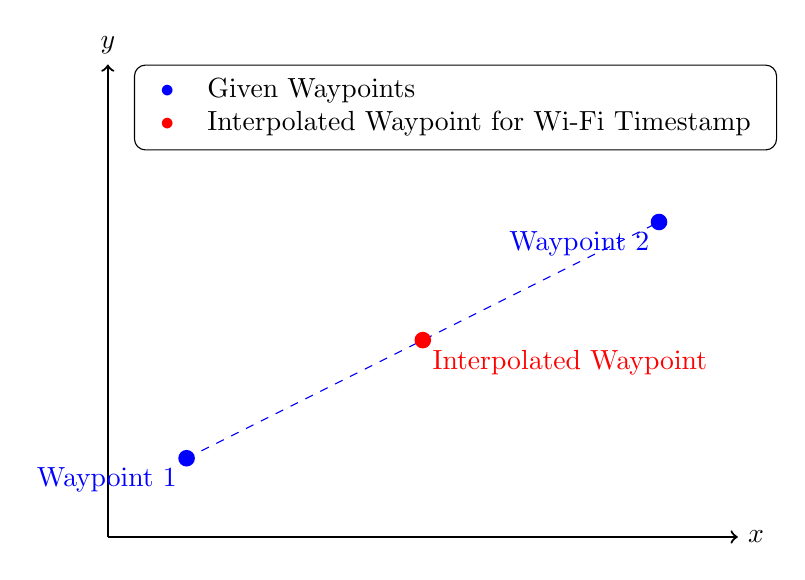
\begin{tikzpicture}
    % Axis
    \draw[->, thick] (0,0) -- (8,0) node[right] {$x$};
    \draw[->, thick] (0,0) -- (0,6) node[above] {$y$};

    % Given Waypoints (e.g., from the waypoints data)
    \fill[blue] (1,1) circle (3pt) node[below left] {Waypoint 1};
    \fill[blue] (7,4) circle (3pt) node[below left] {Waypoint 2};
    \draw[dashed, blue] (1,1) -- (7,4);

    % Interpolated Points (e.g., for wifi_timestamps)
    \fill[red] (4,2.5) circle (3pt) node[below right] {Interpolated Waypoint};

    % Legend
    \node[draw, rectangle, rounded corners, fill=white, anchor=north east] at (8.5,6) {
        \begin{tabular}{c l}
        \color{blue} $\bullet$ & Given Waypoints \\
        \color{red} $\bullet$ & Interpolated Waypoint for Wi-Fi Timestamp \\
        \end{tabular}
    };
\end{tikzpicture}
%     \caption{Visualization of linear interpolation for \ac{wifi} timestamps based on given waypoints. The blue points represent the original waypoints, while the red points show the interpolated positions for specific \ac{wifi}}
%     \label{fig:interpolation}
% \end{figure}

Therefore, an interpolation of \texttt{TYPE\_WAYPOINT} data for \texttt{TYPE\_WIFI} timestamps will be done in order to get a location for the \ac{wifi}.
With this interpolation, we have a combination of \texttt{TYPE\_WAYPOINT} and \texttt{TYPE\_WIFI} data and more data we could use for the prediction.
The interpolation results in 6549 waypoints, three times more than the original waypoints, as seen in \Cref{fig:vis-interpolated}.

\begin{figure}[h!]
    \centering
    \includegraphics[scale=0.375]{images/whole_floor_visualization_interpolated.pdf}
    \caption{Visualization of the interpolated waypoints for site Yintai City (Chengxi Branch) on floor F1}
    \label{fig:vis-interpolated}
\end{figure}

Furthermore, we will also interpolate \texttt{TYPE\_ACCELEROMETER} data for \texttt{TYPE\_WIFI} timestamps because, if the timestamps do not match for \texttt{TYPE\_WIFI} and \texttt{TYPE\_ACCELEROMETER} we will interpolate for a small time range, which may not change the acceleration values significantly and may result in a more accurate prediction.
Now we have a multivariate time series with \texttt{TYPE\_WAYPOINT} and \texttt{TYPE\_ACCELEROMETER} data for \texttt{TYPE\_WIFI} timestamps out of the original data as one file, which will be used for the machine learning model.
Further interpolating the other data, such as \texttt{TYPE\_GYROSCOPE}, is possible, but this thesis only utilizes the abovementioned data.


\subsection{Peculiarities of the data}\label{sec:special-cases}
The dataset analysis revealed some peculiarities, which are described in the following.

Different devices collect the data at different timestamps and days.
A problem for the time series is that the waypoint data were measured irregularly.
As in \Cref{fig:vis-wo-interpolated} shows, some waypoints seem to be very distant from the next one, which can be detected by the dotted lines that go all across the floor.
\Cref{lst:metric-diff} shows the top 10 pairs of waypoints with the most significant metric differences, where \(174.77\) meters is the most significant difference.\\

\begin{lstlisting}[caption={Top 10 pairs with the most significant metric differences of data from floor F1 of site Yintai City (Chengxi Branch)},label={lst:metric-diff}]
    1. Point 1: (247.96523998265695, 168.7631635050295), Point 2: (117.92375106521739, 51.997759545341616), Metric Difference: 174.77113148839442
    2. Point 1: (98.66346, 127.5971), Point 2: (258.75049789436116, 181.23350740899357), Metric Difference: 168.83342057049657
    3. Point 1: (189.58672, 71.454666), Point 2: (89.73448203762376, 102.255128190099), Metric Difference: 104.49467879858156
    4. Point 1: (223.49295, 145.0939), Point 2: (174.26284532732006, 78.86335505811792), Metric Difference: 82.52325908119289
    5. Point 1: (34.864815, 35.45561), Point 2: (33.284438514193546, 110.76117936967742), Metric Difference: 75.32215057954856
    6. Point 1: (50.31085719185683, 92.03105531572366), Point 2: (114.97229034709193, 123.04521228267667), Metric Difference: 71.71456525741291
    7. Point 1: (150.91972285390713, 145.15169976783693), Point 2: (222.23440919809525, 146.11043967333333), Metric Difference: 71.32113060360388
    8. Point 1: (64.64140228107132, 25.345204272946134), Point 2: (34.47475562023909, 84.44615420072283), Metric Difference: 66.35471990088624
    9. Point 1: (56.83799274253731, 74.52090035349569), Point 2: (94.43750948519768, 125.97292215289488), Metric Difference: 63.72624425248555
    10. Point 1: (172.3439286324042, 56.200716101045295), Point 2: (212.4478039192399, 99.33967479470648), Metric Difference: 58.90068395354572
\end{lstlisting}

This difference is too high for a human to walk in \(1.8\) to \(2.2\) seconds, the time between two waypoints.
A human's gait speed has its maximum at about \(2.53\) meters per second, according to \cite{bohannonComfortableMaximumWalking1997}.
So in \(2.2\) seconds, a human can walk \(5.57\) meters, which is much less than each of the values in the top 10 in \Cref{lst:metric-diff}.
Therefore, waypoints, which are more than about 5.57 meters apart, are defined as ``too apart from each other'' to walk in this time, and therefore, we will split the path there and generate separated files.
This results in 147 files with data interpolation, which will be used for the \ac{ml} model.
However, the data in those interpolated files do not contain any information about the \ac{bssid} and corresponding \ac{rssi} values, which are needed for the prediction.
This will be solved in \Cref{sec:wifi-data}.


\subsection{Received Signal Strength Indicators for each timestamp}\label{sec:wifi-data}
It is evident that for a waypoint, we have not all \ac{rssi} values for each \ac{ap} because the \ac{ap} may be out of range.
In order to use the \ac{rssi} in the prediction and treat each \ac{bssid} as a class for the \ac{ml} model, we need to have a \ac{rssi} value for each \ac{ap} for each timestamp.

First, we will gather all \ac{bssid} of the site by iterating over all \ac{wifi} data and save it in one file.
Every line contains the timestamp, and each column header is the \ac{bssid} of the \ac{ap}, and each value of the line is the \ac{rssi} value of the \ac{bssid} at the timestamp.
If an \ac{ap} is absent, we add a very low value \(-999\) into the field. 
Then, we will use this \ac{wifi} file and iterate over each file with interpolated data, and for each timestamp, the \ac{bssid} and the corresponding \ac{rssi} value.
At each timestamp with \texttt{TYPE\_WIFI} timestamps, the \ac{rssi} value for each \ac{bssid} is now saved.
These files will train the \ac{ml} model.
